\documentclass{article}
\renewcommand \thesection{\roman{section}}
\usepackage[utf8]{inputenc}
\usepackage{mathtools}
\usepackage{graphicx}
\usepackage[margin=1in]{geometry}
\usepackage{multicol}
\usepackage{enumitem}
\setlist{nolistsep}
\setlength{\columnsep}{1cm}
\title{AP Physics Notes}
\begin{document}

\begingroup  
  \centering
  \LARGE AP Physics Notes\\[1ex]
  \large Prathmesh Desai\par
\endgroup

\section{Kinematics}
\subsection{Position, Velocity, and Acceleration}
\begin{multicols}{2}

\[\frac{d\vec{x}}{dt}=\vec{v}(t)\]
\[\frac{d^2\vec{x}}{dt^2}=\frac{d\vec{v}}{dt}=\vec{a}(t)\]
\[\bar{v}=\frac{\Delta{x}}{\Delta{t}}\]
\[\bar{a}=\frac{\Delta{v}}{\Delta{t}}\]
\[\vec{v_f}=\vec{v_i}+\vec{a}t\]
\[\vec{d}=\vec{v_i}t+\frac{1}{2}\vec{a}t^2\]
\[\vec{v_f}^2=\vec{v_i}^2+2\vec{a}(\Delta{x})\]
\[g=-9.8\frac{m}{s^2}\]

\columnbreak

Freefall and Projectile Motion:
\vspace{3mm}
\begin{itemize}
\item All free-falling objects do not encounter air resistance\ldots in an ideal world
\item All free-falling objects (on Earth) accelerate downwards at a rate of approximately $9.8\frac{m}{s^2}$
\item All free-falling objects have a constant $v_x$
\item $v_y=0$ \ldots at maximum of y-value of projectile
\end{itemize}

\vspace{2ex}
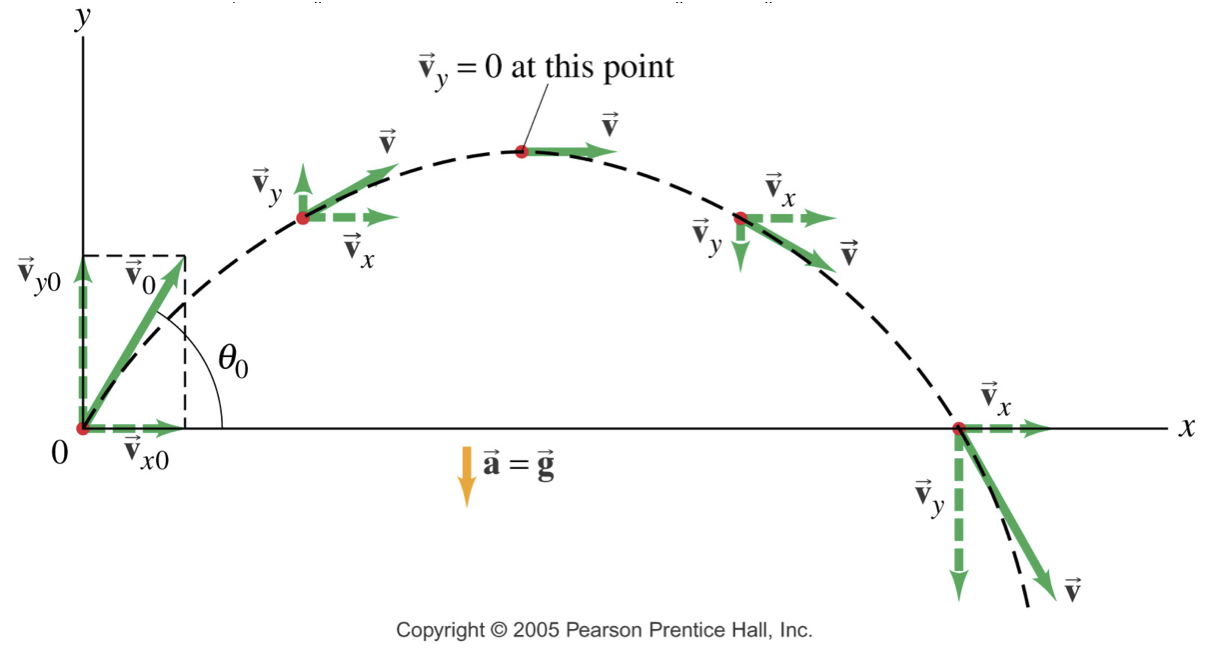
\includegraphics[width=8cm]{ProjectileMotion.jpg}

\end{multicols}

Sample Problems: \vspace{1em}

\begin{multicols}{2}
A loose nail falls from the top of an elevator shaft.  At the same instant 25 m below is the roof of an elevator car rising at a constant 3.0 m/s. \\*\\* Find: \\*
\begin{enumerate}[label=\alph*]
\item Position \\*
\item Velocity of the nail just before it hits the roof of the elevator car\\*
\end{enumerate}
Nail: $v_i$ = 0$\frac{m}{s}$ and $d_y$ = 25m, above elevator\\*
Elevator: $v_i$ = 3$\frac{m}{s}$, up and $d_y$ = 0m

\columnbreak

In time, \textit{t}, the vertical distance travelled equals:

\[\Delta{x_n}=25m-\frac{gt^2}{2} \indent \Delta{x_e}=0m-v_et\]

So \textit{t} is the solution to the equation:

\[25m-\frac{gt^2}{2}=0m-v_et \indent t=1.9733s\]

\begin{enumerate}[label=\alph*]
\item $x=v_et=(-3\frac{m}{s})(1.9733s)=19m,$ up \\*
\item $v_n=gt=(-9.8\frac{m}{s^2})(1.9733s)=19\frac{m}{s},$ down
\end{enumerate}

\end{multicols}

\begin {multicols}{2}
Suppose a volleyball player wants to serve the ball such that it just barely passes over the net.  Let x represent the horizontal distance to the net and y represent the height of the net relative to the launch point of the ball.
\\*\\*
Derive an equation that gives the initial launch angle in terms of x and y.
\columnbreak
\[v_x\]
\end{multicols}

\subsection{Forces and Newton's Laws of Motion}
\subsubsection{Newton's First Law of Motion}

Every object in a state of uniform motion tends to remain in that state of motion unless an external force is applied to it.

\subsubsection{Newton's Second Law of Motion}

The vector sum of the forces $\vec{F}$ on an object is equal to the mass m of that object multiplied by the acceleration $\vec{a}$ of the object.

\[\Sigma\vec{F}=m\vec{a}\]

\subsubsection{Newton's Third Law of Motion}

When one body exerts a force on a second body, the second body simultaneously exerts a force equal in magnitude and opposite in direction on the first body.

\end{document}